\documentclass[11pt]{article}

\usepackage{mathpazo}			%Load palatino font & pazo math
\usepackage{color}	

\usepackage{amsmath, amsthm, amssymb}

\usepackage{tikz}
\usepackage{tikz-3dplot}
\usetikzlibrary{arrows.meta, cd, fadings, patterns}

\usepackage{pgfplots}
\usepackage[inline]{asymptote}

\usepackage{graphicx}
\usepackage{adjustbox}
\usepackage{dsfont}
\usepackage{booktabs}
\usetikzlibrary{decorations.shapes}


\pgfplotsset{compat=1.14}
 
\tikzfading[name=fade out, inner color=transparent!0, outer color=transparent!100]


\begin{document}

% Coffee cup with map out
%%%%%%%%%%%%%%%%%%%%%%%%%%%%%%%%%%%%% 
\begin{tikzpicture}[scale=\textwidth/5cm,samples=200]

% Handle
\begin{scope}[shift=(10:7/8), rotate=-30, yslant=1/2, xslant=-1/8]
  \shade [top color=gray!80, bottom color=gray!30] 
    (0,0) arc (130:-100:3/8 and 1/2) -- ++(0,1/4) arc (-100:130:1/8 and 1/4) -- cycle;
  \shade [top color=gray!10, bottom color=gray!60] 
    (0,0) arc (130:-100:3/8 and 1/2) -- ++(0,1/32) arc (-100:130:1/4 and 1/3) -- cycle;
\end{scope}

% Cup
\fill [black!75, path fading=fade out] 
    (0,-1) ellipse [x radius=3/4, y radius=1/2];
\shade [left color=gray!60, right color=gray!30] 
  (-1,0) arc (180:360:1 and 5/4);
\shade [bottom color=gray, top color=gray!30, opacity=1/2]
  (-1,0) arc (180:360:1 and 5/4);
\shade [left color=gray!20, right color=gray!40] 
  (0,0) ellipse [x radius=1, y radius=1/2];
\shade [left color=gray!40, right color=gray!20] 
  (0,0) ellipse [x radius=1-1/16, y radius=1/2-1/16];
\shade [bottom color=gray, top color=gray!10, opacity=1/2] 
  (0,0) ellipse [x radius=1-1/16, y radius=1/2-1/16];
  
% Coffee Cup Label
\draw  (0,-1.7) node {$X = $ A Coffee Cup};

% Arrow for map
\draw[-{Latex[length=3mm,width=3mm]}] (1.5, -.5) .. controls (2, -1) and (2.5, .5)  ..(4.2, -.5);

% Label for arrow
\draw  (3.0,0) node {$f: X \to Y$};

\end{tikzpicture}
%%%%%%%%%%%%%%%%%%%%%%%%%%%%%%%%%%%%% 


% Torus in R3
% todo: doesn't work
%%%%%%%%%%%%%%%%%%%%%%%%%%%%%%%%%%%%% 
\begin{asy}
  size(400);
  import graph3;

  currentprojection=perspective(5,4,4);
  real R=3;
  real a=1;

  triple fs(pair t) {
    return ((R+a*Cos(t.y))*Cos(t.x),(R+a*Cos(t.y))*Sin(t.x),a*Sin(t.y));
  };

  surface s=surface(fs,(0,180),(360,360),8,8,Spline);
  draw(s,surfacepen=material(blue+opacity(0.6), emissivepen=0.2*white),render(compression=Low,merge=true));

  xaxis3(Label("$x$",1),xmin=0,xmax=7,Arrow3);
  yaxis3(Label("$y$",1),ymin=0,ymax=7,Arrow3);
  zaxis3(Label("$z$",1),zmin=0,zmax=4,Arrow3);
  label("$Y = $ A Torus", (0,-40), p = fontsize(30pt));
\end{asy}
%%%%%%%%%%%%%%%%%%%%%%%%%%%%%%%%%%%%%



% Sphere vs. Ball for Low Dimensions
%%%%%%%%%%%%%%%%%%%%%%%%%%%%%%%%%%%%%
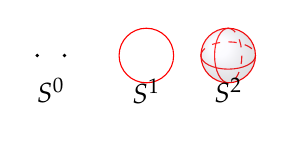
\begin{tikzpicture}[scale=\textwidth/35cm,samples=200]
	\draw (-7,0)[fill=red] circle (.4mm);
	\draw (-6,0)[fill=red] circle (.4mm);
	\draw  (-6.5,-1.3) node {$S^0$};

    \draw[red] (-3,0) circle (1cm);
	\draw  (-3,-1.3) node {$S^1$};
	
	\draw[red] (-1,0) arc (180:360:1cm and 0.5cm);
    \draw[dashed, red] (-1,0) arc (180:0:1cm and 0.5cm);
    \draw[red] (0,1) arc (90:270:0.5cm and 1cm);
    \draw[dashed, red] (0,1) arc (90:-90:0.5cm and 1cm);
    \draw[red] (0,0) circle (1cm);
    \shade[ball color=blue!10!white,opacity=0.20] (0,0) circle (1cm);
    \draw  (0,-1.3) node {$S^2$};
\end{tikzpicture}

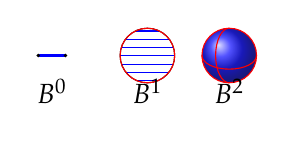
\begin{tikzpicture}[scale=\textwidth/35cm,samples=200]
	\draw[thick, blue] (-7,0) -- (-6,0);
	\draw[fill=red](-6,0) circle (.4mm);
	\draw[fill=red](-7,0) circle (.4mm);
	\draw (-6.5,-1.3) node {$B^0$};

	%\shade[ball color=blue!100!white] (-3,0) circle (1cm);
	\draw[pattern=horizontal lines, pattern color=blue] (-3,0) circle (1cm);
    \draw[red] (-3,0) circle (1cm);
	\draw (-3,-1.3) node {$B^1$};

    \shade[ball color=blue!100!white,opacity=0.90] (0,0) circle (1cm);
    \draw[red] (0,0) circle (1cm);
   	\draw[red] (-1,0) arc (180:360:1cm and 0.5cm);
    \draw[red] (0,1) arc (90:270:0.5cm and 1cm);
    \draw  (0,-1.3) node {$B^2$};
\end{tikzpicture}
%%%%%%%%%%%%%%%%%%%%%%%%%%%%%%%%%%%%%

\end{document}
